\documentclass[twoside]{book}

% Packages required by doxygen
\usepackage{fixltx2e}
\usepackage{calc}
\usepackage{doxygen}
\usepackage[export]{adjustbox} % also loads graphicx
\usepackage{graphicx}
\usepackage[utf8]{inputenc}
\usepackage{makeidx}
\usepackage{multicol}
\usepackage{multirow}
\PassOptionsToPackage{warn}{textcomp}
\usepackage{textcomp}
\usepackage[nointegrals]{wasysym}
\usepackage[table]{xcolor}

% NLS support packages
\usepackage[french]{babel}

% Font selection
\usepackage[T1]{fontenc}
\usepackage[scaled=.90]{helvet}
\usepackage{courier}
\usepackage{amssymb}
\usepackage{sectsty}
\renewcommand{\familydefault}{\sfdefault}
\allsectionsfont{%
  \fontseries{bc}\selectfont%
  \color{darkgray}%
}
\renewcommand{\DoxyLabelFont}{%
  \fontseries{bc}\selectfont%
  \color{darkgray}%
}
\newcommand{\+}{\discretionary{\mbox{\scriptsize$\hookleftarrow$}}{}{}}

% Page & text layout
\usepackage{geometry}
\geometry{%
  a4paper,%
  top=2.5cm,%
  bottom=2.5cm,%
  left=2.5cm,%
  right=2.5cm%
}
\tolerance=750
\hfuzz=15pt
\hbadness=750
\setlength{\emergencystretch}{15pt}
\setlength{\parindent}{0cm}
\setlength{\parskip}{3ex plus 2ex minus 2ex}
\makeatletter
\renewcommand{\paragraph}{%
  \@startsection{paragraph}{4}{0ex}{-1.0ex}{1.0ex}{%
    \normalfont\normalsize\bfseries\SS@parafont%
  }%
}
\renewcommand{\subparagraph}{%
  \@startsection{subparagraph}{5}{0ex}{-1.0ex}{1.0ex}{%
    \normalfont\normalsize\bfseries\SS@subparafont%
  }%
}
\makeatother

% Headers & footers
\usepackage{fancyhdr}
\pagestyle{fancyplain}
\fancyhead[LE]{\fancyplain{}{\bfseries\thepage}}
\fancyhead[CE]{\fancyplain{}{}}
\fancyhead[RE]{\fancyplain{}{\bfseries\leftmark}}
\fancyhead[LO]{\fancyplain{}{\bfseries\rightmark}}
\fancyhead[CO]{\fancyplain{}{}}
\fancyhead[RO]{\fancyplain{}{\bfseries\thepage}}
\fancyfoot[LE]{\fancyplain{}{}}
\fancyfoot[CE]{\fancyplain{}{}}
\fancyfoot[RE]{\fancyplain{}{\bfseries\scriptsize Généré par Doxygen }}
\fancyfoot[LO]{\fancyplain{}{\bfseries\scriptsize Généré par Doxygen }}
\fancyfoot[CO]{\fancyplain{}{}}
\fancyfoot[RO]{\fancyplain{}{}}
\renewcommand{\footrulewidth}{0.4pt}
\renewcommand{\chaptermark}[1]{%
  \markboth{#1}{}%
}
\renewcommand{\sectionmark}[1]{%
  \markright{\thesection\ #1}%
}

% Indices & bibliography
\usepackage{natbib}
\usepackage[titles]{tocloft}
\setcounter{tocdepth}{3}
\setcounter{secnumdepth}{5}
\makeindex

% Hyperlinks (required, but should be loaded last)
\usepackage{ifpdf}
\ifpdf
  \usepackage[pdftex,pagebackref=true]{hyperref}
\else
  \usepackage[ps2pdf,pagebackref=true]{hyperref}
\fi
\hypersetup{%
  colorlinks=true,%
  linkcolor=blue,%
  citecolor=blue,%
  unicode%
}

% Custom commands
\newcommand{\clearemptydoublepage}{%
  \newpage{\pagestyle{empty}\cleardoublepage}%
}

\usepackage{caption}
\captionsetup{labelsep=space,justification=centering,font={bf},singlelinecheck=off,skip=4pt,position=top}

%===== C O N T E N T S =====

\begin{document}

% Titlepage & ToC
\hypersetup{pageanchor=false,
             bookmarksnumbered=true,
             pdfencoding=unicode
            }
\pagenumbering{roman}
\begin{titlepage}
\vspace*{7cm}
\begin{center}%
{\Large Moniteur\+Roomba }\\
\vspace*{1cm}
{\large Généré par Doxygen 1.8.11}\\
\end{center}
\end{titlepage}
\clearemptydoublepage
\tableofcontents
\clearemptydoublepage
\pagenumbering{arabic}
\hypersetup{pageanchor=true}

%--- Begin generated contents ---
\chapter{Index des espaces de nommage}
\section{Liste des espaces de nommage}
Liste de tous les espaces de nommage documentés avec une brève description\+:\begin{DoxyCompactList}
\item\contentsline{section}{\hyperlink{namespace_ui}{Ui} }{\pageref{namespace_ui}}{}
\end{DoxyCompactList}

\chapter{Index hiérarchique}
\section{Hiérarchie des classes}
Cette liste d\textquotesingle{}héritage est classée approximativement par ordre alphabétique \+:\begin{DoxyCompactList}
\item \contentsline{section}{Config\+Liaison}{\pageref{class_config_liaison}}{}
\item \contentsline{section}{Liaison}{\pageref{class_liaison}}{}
\item Q\+Main\+Window\begin{DoxyCompactList}
\item \contentsline{section}{Main\+Window}{\pageref{class_main_window}}{}
\end{DoxyCompactList}
\item \contentsline{section}{Trame}{\pageref{class_trame}}{}
\end{DoxyCompactList}

\chapter{Index des classes}
\section{Liste des classes}
Liste des classes, structures, unions et interfaces avec une brève description \+:\begin{DoxyCompactList}
\item\contentsline{section}{\hyperlink{class_config_liaison}{Config\+Liaison} \\*Cette classe définit les paramètres de la liaison. En première approche, seule la liaison série est envisagée. Les attributs de la classe sont les paramètres de la liaison série }{\pageref{class_config_liaison}}{}
\item\contentsline{section}{\hyperlink{class_liaison}{Liaison} \\*Réalise la communication avec le Roomba }{\pageref{class_liaison}}{}
\item\contentsline{section}{\hyperlink{class_main_window}{Main\+Window} }{\pageref{class_main_window}}{}
\item\contentsline{section}{\hyperlink{class_trame}{Trame} \\*Stocke une trame comme suite d\textquotesingle{}octets, et permet d\textquotesingle{}extraire des valeurs à une poistion et selon un format donné, suivant les types employés dans le protocole R\+OI }{\pageref{class_trame}}{}
\end{DoxyCompactList}

\chapter{Index des fichiers}
\section{Liste des fichiers}
Liste de tous les fichiers documentés avec une brève description \+:\begin{DoxyCompactList}
\item\contentsline{section}{/home/\+I\+R/fortin/\+Moniteur\+Roomba/{\bfseries configliaison.\+cpp} }{\pageref{configliaison_8cpp}}{}
\item\contentsline{section}{/home/\+I\+R/fortin/\+Moniteur\+Roomba/\hyperlink{_config_liaison_8h}{Config\+Liaison.\+h} }{\pageref{_config_liaison_8h}}{}
\item\contentsline{section}{/home/\+I\+R/fortin/\+Moniteur\+Roomba/{\bfseries Liaison.\+cpp} }{\pageref{_liaison_8cpp}}{}
\item\contentsline{section}{/home/\+I\+R/fortin/\+Moniteur\+Roomba/\hyperlink{_liaison_8h}{Liaison.\+h} }{\pageref{_liaison_8h}}{}
\item\contentsline{section}{/home/\+I\+R/fortin/\+Moniteur\+Roomba/{\bfseries main.\+cpp} }{\pageref{main_8cpp}}{}
\item\contentsline{section}{/home/\+I\+R/fortin/\+Moniteur\+Roomba/{\bfseries mainwindow.\+cpp} }{\pageref{mainwindow_8cpp}}{}
\item\contentsline{section}{/home/\+I\+R/fortin/\+Moniteur\+Roomba/{\bfseries mainwindow.\+h} }{\pageref{mainwindow_8h}}{}
\item\contentsline{section}{/home/\+I\+R/fortin/\+Moniteur\+Roomba/{\bfseries Trame.\+cpp} }{\pageref{_trame_8cpp}}{}
\item\contentsline{section}{/home/\+I\+R/fortin/\+Moniteur\+Roomba/\hyperlink{_trame_8h}{Trame.\+h} }{\pageref{_trame_8h}}{}
\end{DoxyCompactList}

\chapter{Documentation des espaces de nommage}
\hypertarget{namespace_ui}{}\section{Référence de l\textquotesingle{}espace de nommage Ui}
\label{namespace_ui}\index{Ui@{Ui}}


\subsection{Description détaillée}
file copyright L\+G\+PL v3 date 14/09/2017 author F\+O\+R\+T\+IN Pierre 
\chapter{Documentation des classes}
\hypertarget{class_config_liaison}{}\section{Référence de la classe Config\+Liaison}
\label{class_config_liaison}\index{Config\+Liaison@{Config\+Liaison}}


Cette classe définit les paramètres de la liaison. En première approche, seule la liaison série est envisagée. Les attributs de la classe sont les paramètres de la liaison série.  




{\ttfamily \#include $<$Config\+Liaison.\+h$>$}

\subsection*{Fonctions membres publiques}
\begin{DoxyCompactItemize}
\item 
Q\+String {\bfseries port} () const \hypertarget{class_config_liaison_ae1fd90dc7c1003f0d0515435f32cac7b}{}\label{class_config_liaison_ae1fd90dc7c1003f0d0515435f32cac7b}

\item 
int {\bfseries debit} () const \hypertarget{class_config_liaison_a7966350b65217586e89460eb3c7f74d6}{}\label{class_config_liaison_a7966350b65217586e89460eb3c7f74d6}

\item 
void {\bfseries set\+Port} (Q\+String port)\hypertarget{class_config_liaison_a76ff36009aac38bd0bb4b72de76e34c9}{}\label{class_config_liaison_a76ff36009aac38bd0bb4b72de76e34c9}

\item 
void {\bfseries set\+Debit} (int debit)\hypertarget{class_config_liaison_a9859103f842682698d2a5660807514fc}{}\label{class_config_liaison_a9859103f842682698d2a5660807514fc}

\end{DoxyCompactItemize}
\subsection*{Attributs privés}
\begin{DoxyCompactItemize}
\item 
Q\+String \hyperlink{class_config_liaison_a605dab2080bf9d7944edf7146dc23d3c}{m\+Port}\hypertarget{class_config_liaison_a605dab2080bf9d7944edf7146dc23d3c}{}\label{class_config_liaison_a605dab2080bf9d7944edf7146dc23d3c}

\begin{DoxyCompactList}\small\item\em Le nom de port de communication. \end{DoxyCompactList}\item 
int \hyperlink{class_config_liaison_aed444290c04caf89c334e9b871d61b96}{m\+Debit}\hypertarget{class_config_liaison_aed444290c04caf89c334e9b871d61b96}{}\label{class_config_liaison_aed444290c04caf89c334e9b871d61b96}

\begin{DoxyCompactList}\small\item\em Le débit de communication en baud. \end{DoxyCompactList}\end{DoxyCompactItemize}


\subsection{Description détaillée}
Cette classe définit les paramètres de la liaison. En première approche, seule la liaison série est envisagée. Les attributs de la classe sont les paramètres de la liaison série. 

Définition à la ligne 18 du fichier Config\+Liaison.\+h.



La documentation de cette classe a été générée à partir des fichiers suivants \+:\begin{DoxyCompactItemize}
\item 
/home/\+I\+R/fortin/\+Moniteur\+Roomba/\hyperlink{_config_liaison_8h}{Config\+Liaison.\+h}\item 
/home/\+I\+R/fortin/\+Moniteur\+Roomba/configliaison.\+cpp\end{DoxyCompactItemize}

\hypertarget{class_liaison}{}\section{Référence de la classe Liaison}
\label{class_liaison}\index{Liaison@{Liaison}}


Réalise la communication avec le Roomba.  




{\ttfamily \#include $<$Liaison.\+h$>$}

\subsection*{Fonctions membres publiques}
\begin{DoxyCompactItemize}
\item 
bool {\bfseries Connexion\+Etablie} () const \hypertarget{class_liaison_adf5c86d29003736af1e06adb94c58d65}{}\label{class_liaison_adf5c86d29003736af1e06adb94c58d65}

\item 
void \hyperlink{class_liaison_adbccfcb0fd523be8dc4eb46bfb36f082}{configurer} (\hyperlink{class_config_liaison}{Config\+Liaison} cfg)
\begin{DoxyCompactList}\small\item\em Définir la configuration de la liaison. \end{DoxyCompactList}\item 
bool \hyperlink{class_liaison_ad760074370ae78ba996ccc1c2c85b91d}{connecter} ()
\begin{DoxyCompactList}\small\item\em Établir la connexion au Roomba. \end{DoxyCompactList}\item 
bool \hyperlink{class_liaison_a04b34111e5c80a2f429ac5209e7597b7}{deconnecter} ()
\begin{DoxyCompactList}\small\item\em Refermer la connexion au Roomba. \end{DoxyCompactList}\item 
void \hyperlink{class_liaison_ab1e3ee8df9a7930635950a3a04f1579c}{envoyer\+Commande} (Q\+Byte\+Array commande)
\begin{DoxyCompactList}\small\item\em Envoyer au Roomba une commande. \end{DoxyCompactList}\item 
\hyperlink{class_trame}{Trame} \hyperlink{class_liaison_aac991944c85ac165fcb6c213a2449313}{lire\+Trame} ()
\begin{DoxyCompactList}\small\item\em Lire la trame envoyée par le Roomba. \end{DoxyCompactList}\end{DoxyCompactItemize}
\subsection*{Attributs privés}
\begin{DoxyCompactItemize}
\item 
\hyperlink{class_config_liaison}{Config\+Liaison} \hyperlink{class_liaison_a0357bc6671680d6b495fe25ce6d2b128}{m\+Cfg}\hypertarget{class_liaison_a0357bc6671680d6b495fe25ce6d2b128}{}\label{class_liaison_a0357bc6671680d6b495fe25ce6d2b128}

\begin{DoxyCompactList}\small\item\em m\+Cfg La configuration de la liaison \end{DoxyCompactList}\item 
Q\+Serial\+Port \hyperlink{class_liaison_a94a391d4b617c092e4cc3fd1d4397a6c}{m\+LS}\hypertarget{class_liaison_a94a391d4b617c092e4cc3fd1d4397a6c}{}\label{class_liaison_a94a391d4b617c092e4cc3fd1d4397a6c}

\begin{DoxyCompactList}\small\item\em m\+LS Accès au port de communication série \end{DoxyCompactList}\item 
bool \hyperlink{class_liaison_a9832b59d823545937decd984070c461e}{m\+Connexion\+Etablie}\hypertarget{class_liaison_a9832b59d823545937decd984070c461e}{}\label{class_liaison_a9832b59d823545937decd984070c461e}

\begin{DoxyCompactList}\small\item\em m\+Connexion\+Etablie L\textquotesingle{}état de la liaison \+: true lors de la connexion au Roomba est réalisée. \end{DoxyCompactList}\end{DoxyCompactItemize}


\subsection{Description détaillée}
Réalise la communication avec le Roomba. 

Elle réalise la configuration, l\textquotesingle{}ouverture et la ermeture de la connexion. Elle gère la réception de trames suivant le protocole R\+OI (Roomba Open Interface). 

Définition à la ligne 21 du fichier Liaison.\+h.



\subsection{Documentation des fonctions membres}
\index{Liaison@{Liaison}!configurer@{configurer}}
\index{configurer@{configurer}!Liaison@{Liaison}}
\subsubsection[{\texorpdfstring{configurer(\+Config\+Liaison cfg)}{configurer(ConfigLiaison cfg)}}]{\setlength{\rightskip}{0pt plus 5cm}void Liaison\+::configurer (
\begin{DoxyParamCaption}
\item[{{\bf Config\+Liaison}}]{cfg}
\end{DoxyParamCaption}
)}\hypertarget{class_liaison_adbccfcb0fd523be8dc4eb46bfb36f082}{}\label{class_liaison_adbccfcb0fd523be8dc4eb46bfb36f082}


Définir la configuration de la liaison. 


\begin{DoxyParams}{Paramètres}
{\em cfg} & La configuration de la liaison \\
\hline
\end{DoxyParams}


Définition à la ligne 3 du fichier Liaison.\+cpp.

\index{Liaison@{Liaison}!connecter@{connecter}}
\index{connecter@{connecter}!Liaison@{Liaison}}
\subsubsection[{\texorpdfstring{connecter()}{connecter()}}]{\setlength{\rightskip}{0pt plus 5cm}bool Liaison\+::connecter (
\begin{DoxyParamCaption}
{}
\end{DoxyParamCaption}
)}\hypertarget{class_liaison_ad760074370ae78ba996ccc1c2c85b91d}{}\label{class_liaison_ad760074370ae78ba996ccc1c2c85b91d}


Établir la connexion au Roomba. 

\begin{DoxyReturn}{Renvoie}
Retour\+: True si la connexion est réalisée 
\end{DoxyReturn}


Définition à la ligne 8 du fichier Liaison.\+cpp.

\index{Liaison@{Liaison}!deconnecter@{deconnecter}}
\index{deconnecter@{deconnecter}!Liaison@{Liaison}}
\subsubsection[{\texorpdfstring{deconnecter()}{deconnecter()}}]{\setlength{\rightskip}{0pt plus 5cm}bool Liaison\+::deconnecter (
\begin{DoxyParamCaption}
{}
\end{DoxyParamCaption}
)}\hypertarget{class_liaison_a04b34111e5c80a2f429ac5209e7597b7}{}\label{class_liaison_a04b34111e5c80a2f429ac5209e7597b7}


Refermer la connexion au Roomba. 

\begin{DoxyReturn}{Renvoie}
Retour\+: True si la connexion est refermée 
\end{DoxyReturn}


Définition à la ligne 13 du fichier Liaison.\+cpp.

\index{Liaison@{Liaison}!envoyer\+Commande@{envoyer\+Commande}}
\index{envoyer\+Commande@{envoyer\+Commande}!Liaison@{Liaison}}
\subsubsection[{\texorpdfstring{envoyer\+Commande(\+Q\+Byte\+Array commande)}{envoyerCommande(QByteArray commande)}}]{\setlength{\rightskip}{0pt plus 5cm}void Liaison\+::envoyer\+Commande (
\begin{DoxyParamCaption}
\item[{Q\+Byte\+Array}]{commande}
\end{DoxyParamCaption}
)}\hypertarget{class_liaison_ab1e3ee8df9a7930635950a3a04f1579c}{}\label{class_liaison_ab1e3ee8df9a7930635950a3a04f1579c}


Envoyer au Roomba une commande. 


\begin{DoxyParams}{Paramètres}
{\em Paramètre} & commande\+: La commande a envoyer \\
\hline
\end{DoxyParams}


Définition à la ligne 17 du fichier Liaison.\+cpp.

\index{Liaison@{Liaison}!lire\+Trame@{lire\+Trame}}
\index{lire\+Trame@{lire\+Trame}!Liaison@{Liaison}}
\subsubsection[{\texorpdfstring{lire\+Trame()}{lireTrame()}}]{\setlength{\rightskip}{0pt plus 5cm}{\bf Trame} Liaison\+::lire\+Trame (
\begin{DoxyParamCaption}
{}
\end{DoxyParamCaption}
)}\hypertarget{class_liaison_aac991944c85ac165fcb6c213a2449313}{}\label{class_liaison_aac991944c85ac165fcb6c213a2449313}


Lire la trame envoyée par le Roomba. 

\begin{DoxyReturn}{Renvoie}
Retour\+: La trame obtenue 
\end{DoxyReturn}


Définition à la ligne 21 du fichier Liaison.\+cpp.



La documentation de cette classe a été générée à partir des fichiers suivants \+:\begin{DoxyCompactItemize}
\item 
/home/\+I\+R/fortin/\+Moniteur\+Roomba/\hyperlink{_liaison_8h}{Liaison.\+h}\item 
/home/\+I\+R/fortin/\+Moniteur\+Roomba/Liaison.\+cpp\end{DoxyCompactItemize}

\hypertarget{class_main_window}{}\section{Référence de la classe Main\+Window}
\label{class_main_window}\index{Main\+Window@{Main\+Window}}
Graphe d\textquotesingle{}héritage de Main\+Window\+:\begin{figure}[H]
\begin{center}
\leavevmode
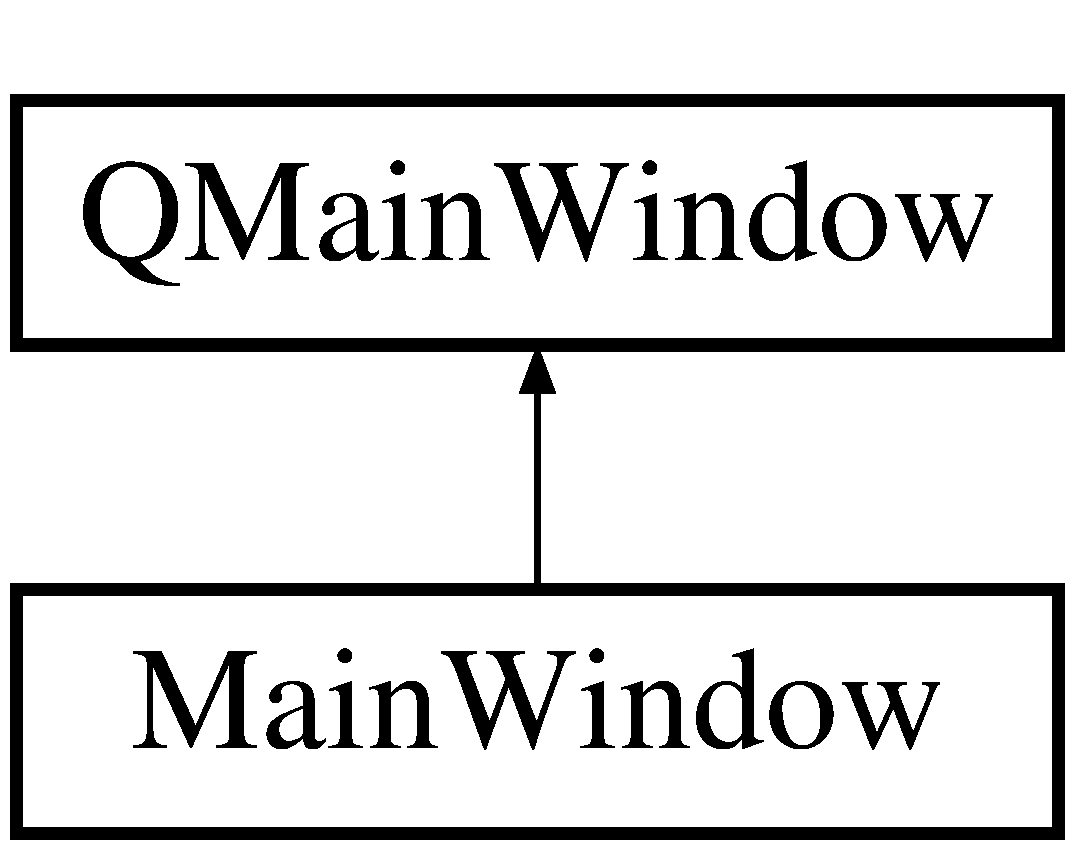
\includegraphics[height=2.000000cm]{class_main_window}
\end{center}
\end{figure}
\subsection*{Fonctions membres publiques}
\begin{DoxyCompactItemize}
\item 
{\bfseries Main\+Window} (Q\+Widget $\ast$parent=0)\hypertarget{class_main_window_a8b244be8b7b7db1b08de2a2acb9409db}{}\label{class_main_window_a8b244be8b7b7db1b08de2a2acb9409db}

\end{DoxyCompactItemize}
\subsection*{Attributs privés}
\begin{DoxyCompactItemize}
\item 
Ui\+::\+Main\+Window $\ast$ {\bfseries ui}\hypertarget{class_main_window_a35466a70ed47252a0191168126a352a5}{}\label{class_main_window_a35466a70ed47252a0191168126a352a5}

\end{DoxyCompactItemize}


\subsection{Description détaillée}


Définition à la ligne 16 du fichier mainwindow.\+h.



La documentation de cette classe a été générée à partir des fichiers suivants \+:\begin{DoxyCompactItemize}
\item 
/home/\+I\+R/fortin/\+Moniteur\+Roomba/mainwindow.\+h\item 
/home/\+I\+R/fortin/\+Moniteur\+Roomba/mainwindow.\+cpp\end{DoxyCompactItemize}

\hypertarget{class_trame}{}\section{Référence de la classe Trame}
\label{class_trame}\index{Trame@{Trame}}


Stocke une trame comme suite d\textquotesingle{}octets, et permet d\textquotesingle{}extraire des valeurs à une poistion et selon un format donné, suivant les types employés dans le protocole R\+OI.  




{\ttfamily \#include $<$Trame.\+h$>$}

\subsection*{Fonctions membres publiques}
\begin{DoxyCompactItemize}
\item 
qint32 \hyperlink{class_trame_a4f27e756e28a3f6031266b2915ad8f5f}{get\+Bit} (quint8 pos, quint8 bit)
\begin{DoxyCompactList}\small\item\em Extrait de la trame la valeur d’un bit. \end{DoxyCompactList}\item 
qint32 \hyperlink{class_trame_a9ad6bf3df1cf43d66571df3db1018056}{get\+Unsigned\+Byte} (quint8 pos)
\begin{DoxyCompactList}\small\item\em Extrait de la trame un octet non signé \end{DoxyCompactList}\item 
qint32 \hyperlink{class_trame_a183f007c20410a5c0cbf2093a02e42f8}{get\+Signed\+Byte} (quint8 pos)
\begin{DoxyCompactList}\small\item\em Extrait de la trame un octet signé \end{DoxyCompactList}\item 
qint32 \hyperlink{class_trame_acedfebffa3d8af24219e5460d4f597de}{get\+Unsigned\+Word} (quint8 pos)
\begin{DoxyCompactList}\small\item\em Extrait de la trame un mot 16 bit non signé \end{DoxyCompactList}\item 
qint32 \hyperlink{class_trame_afcb503453b50b388035e3c4ae0b606b9}{get\+Signed\+Word} (quint8 pos)
\begin{DoxyCompactList}\small\item\em Extrait de la trame un mot 16 bit signé, en réalisant l’extension de signe sur 32 bits. \end{DoxyCompactList}\end{DoxyCompactItemize}


\subsection{Description détaillée}
Stocke une trame comme suite d\textquotesingle{}octets, et permet d\textquotesingle{}extraire des valeurs à une poistion et selon un format donné, suivant les types employés dans le protocole R\+OI. 

Définition à la ligne 17 du fichier Trame.\+h.



\subsection{Documentation des fonctions membres}
\index{Trame@{Trame}!get\+Bit@{get\+Bit}}
\index{get\+Bit@{get\+Bit}!Trame@{Trame}}
\subsubsection[{\texorpdfstring{get\+Bit(quint8 pos, quint8 bit)}{getBit(quint8 pos, quint8 bit)}}]{\setlength{\rightskip}{0pt plus 5cm}qint32 Trame\+::get\+Bit (
\begin{DoxyParamCaption}
\item[{quint8}]{pos, }
\item[{quint8}]{bit}
\end{DoxyParamCaption}
)}\hypertarget{class_trame_a4f27e756e28a3f6031266b2915ad8f5f}{}\label{class_trame_a4f27e756e28a3f6031266b2915ad8f5f}


Extrait de la trame la valeur d’un bit. 


\begin{DoxyParams}{Paramètres}
{\em pos} & L\textquotesingle{}adresse de l\textquotesingle{}octet dans la trame \\
\hline
{\em bit} & Le rang du bit à extraire (en commençant à 0 pour le L\+SB) \\
\hline
\end{DoxyParams}
\begin{DoxyReturn}{Renvoie}
Retour\+: La valeur du bit désigné 
\end{DoxyReturn}


Définition à la ligne 3 du fichier Trame.\+cpp.

\index{Trame@{Trame}!get\+Signed\+Byte@{get\+Signed\+Byte}}
\index{get\+Signed\+Byte@{get\+Signed\+Byte}!Trame@{Trame}}
\subsubsection[{\texorpdfstring{get\+Signed\+Byte(quint8 pos)}{getSignedByte(quint8 pos)}}]{\setlength{\rightskip}{0pt plus 5cm}qint32 Trame\+::get\+Signed\+Byte (
\begin{DoxyParamCaption}
\item[{quint8}]{pos}
\end{DoxyParamCaption}
)}\hypertarget{class_trame_a183f007c20410a5c0cbf2093a02e42f8}{}\label{class_trame_a183f007c20410a5c0cbf2093a02e42f8}


Extrait de la trame un octet signé 


\begin{DoxyParams}{Paramètres}
{\em pos} & L\textquotesingle{}adresse de l\textquotesingle{}octet dans la trame, en réalisant l’extension de signe sur 32 bits \\
\hline
\end{DoxyParams}
\begin{DoxyReturn}{Renvoie}
Retour\+: La valeur de l’octet à la position spécifié 
\end{DoxyReturn}


Définition à la ligne 11 du fichier Trame.\+cpp.

\index{Trame@{Trame}!get\+Signed\+Word@{get\+Signed\+Word}}
\index{get\+Signed\+Word@{get\+Signed\+Word}!Trame@{Trame}}
\subsubsection[{\texorpdfstring{get\+Signed\+Word(quint8 pos)}{getSignedWord(quint8 pos)}}]{\setlength{\rightskip}{0pt plus 5cm}qint32 Trame\+::get\+Signed\+Word (
\begin{DoxyParamCaption}
\item[{quint8}]{pos}
\end{DoxyParamCaption}
)}\hypertarget{class_trame_afcb503453b50b388035e3c4ae0b606b9}{}\label{class_trame_afcb503453b50b388035e3c4ae0b606b9}


Extrait de la trame un mot 16 bit signé, en réalisant l’extension de signe sur 32 bits. 


\begin{DoxyParams}{Paramètres}
{\em pos} & L\textquotesingle{}adresse du 1er octet dans la trame \\
\hline
\end{DoxyParams}
\begin{DoxyReturn}{Renvoie}
Retour\+: Le mot formé par \mbox{[}pos\mbox{]} (M\+SB) et \mbox{[}pos+1\mbox{]} (L\+SB) 
\end{DoxyReturn}


Définition à la ligne 19 du fichier Trame.\+cpp.

\index{Trame@{Trame}!get\+Unsigned\+Byte@{get\+Unsigned\+Byte}}
\index{get\+Unsigned\+Byte@{get\+Unsigned\+Byte}!Trame@{Trame}}
\subsubsection[{\texorpdfstring{get\+Unsigned\+Byte(quint8 pos)}{getUnsignedByte(quint8 pos)}}]{\setlength{\rightskip}{0pt plus 5cm}qint32 Trame\+::get\+Unsigned\+Byte (
\begin{DoxyParamCaption}
\item[{quint8}]{pos}
\end{DoxyParamCaption}
)}\hypertarget{class_trame_a9ad6bf3df1cf43d66571df3db1018056}{}\label{class_trame_a9ad6bf3df1cf43d66571df3db1018056}


Extrait de la trame un octet non signé 


\begin{DoxyParams}{Paramètres}
{\em pos} & L\textquotesingle{}adresse de l\textquotesingle{}octet dans la trame \\
\hline
\end{DoxyParams}
\begin{DoxyReturn}{Renvoie}
Retour\+: La veleur de l\textquotesingle{}octet à la position spécifiée 
\end{DoxyReturn}


Définition à la ligne 7 du fichier Trame.\+cpp.

\index{Trame@{Trame}!get\+Unsigned\+Word@{get\+Unsigned\+Word}}
\index{get\+Unsigned\+Word@{get\+Unsigned\+Word}!Trame@{Trame}}
\subsubsection[{\texorpdfstring{get\+Unsigned\+Word(quint8 pos)}{getUnsignedWord(quint8 pos)}}]{\setlength{\rightskip}{0pt plus 5cm}qint32 Trame\+::get\+Unsigned\+Word (
\begin{DoxyParamCaption}
\item[{quint8}]{pos}
\end{DoxyParamCaption}
)}\hypertarget{class_trame_acedfebffa3d8af24219e5460d4f597de}{}\label{class_trame_acedfebffa3d8af24219e5460d4f597de}


Extrait de la trame un mot 16 bit non signé 


\begin{DoxyParams}{Paramètres}
{\em pos} & L\textquotesingle{}adresse du 1er octet dans la trame \\
\hline
\end{DoxyParams}
\begin{DoxyReturn}{Renvoie}
Retour\+: Le mot formé par \mbox{[}pos\mbox{]} (M\+SB) et \mbox{[}pos+1\mbox{]} (L\+SB) 
\end{DoxyReturn}


Définition à la ligne 15 du fichier Trame.\+cpp.



La documentation de cette classe a été générée à partir des fichiers suivants \+:\begin{DoxyCompactItemize}
\item 
/home/\+I\+R/fortin/\+Moniteur\+Roomba/\hyperlink{_trame_8h}{Trame.\+h}\item 
/home/\+I\+R/fortin/\+Moniteur\+Roomba/Trame.\+cpp\end{DoxyCompactItemize}

\chapter{Documentation des fichiers}
\hypertarget{_config_liaison_8h}{}\section{Référence du fichier /home/\+I\+R/fortin/\+Moniteur\+Roomba/\+Config\+Liaison.h}
\label{_config_liaison_8h}\index{/home/\+I\+R/fortin/\+Moniteur\+Roomba/\+Config\+Liaison.\+h@{/home/\+I\+R/fortin/\+Moniteur\+Roomba/\+Config\+Liaison.\+h}}
{\ttfamily \#include $<$Q\+String$>$}\\*
\subsection*{Classes}
\begin{DoxyCompactItemize}
\item 
class \hyperlink{class_config_liaison}{Config\+Liaison}
\begin{DoxyCompactList}\small\item\em Cette classe définit les paramètres de la liaison. En première approche, seule la liaison série est envisagée. Les attributs de la classe sont les paramètres de la liaison série. \end{DoxyCompactList}\end{DoxyCompactItemize}


\subsection{Description détaillée}
\begin{DoxyCopyright}{Copyright}
L\+G\+PL v3 
\end{DoxyCopyright}
\begin{DoxyDate}{Date}
14/09/2017 
\end{DoxyDate}
\begin{DoxyAuthor}{Auteur}
F\+O\+R\+T\+IN Pierre 
\end{DoxyAuthor}

\hypertarget{_liaison_8h}{}\section{Référence du fichier /home/\+I\+R/fortin/\+Moniteur\+Roomba/\+Liaison.h}
\label{_liaison_8h}\index{/home/\+I\+R/fortin/\+Moniteur\+Roomba/\+Liaison.\+h@{/home/\+I\+R/fortin/\+Moniteur\+Roomba/\+Liaison.\+h}}
{\ttfamily \#include $<$Qt\+Serial\+Port/\+Qt\+Serial\+Port$>$}\\*
{\ttfamily \#include \char`\"{}Config\+Liaison.\+h\char`\"{}}\\*
{\ttfamily \#include \char`\"{}Trame.\+h\char`\"{}}\\*
\subsection*{Classes}
\begin{DoxyCompactItemize}
\item 
class \hyperlink{class_liaison}{Liaison}
\begin{DoxyCompactList}\small\item\em Réalise la communication avec le Roomba. \end{DoxyCompactList}\end{DoxyCompactItemize}


\subsection{Description détaillée}
\begin{DoxyCopyright}{Copyright}
L\+G\+PL v3 
\end{DoxyCopyright}
\begin{DoxyDate}{Date}
14/09/2017 
\end{DoxyDate}
\begin{DoxyAuthor}{Auteur}
F\+O\+R\+T\+IN Pierre 
\end{DoxyAuthor}

\hypertarget{_trame_8h}{}\section{Référence du fichier /home/\+I\+R/fortin/\+Moniteur\+Roomba/\+Trame.h}
\label{_trame_8h}\index{/home/\+I\+R/fortin/\+Moniteur\+Roomba/\+Trame.\+h@{/home/\+I\+R/fortin/\+Moniteur\+Roomba/\+Trame.\+h}}
{\ttfamily \#include $<$Qt\+Global$>$}\\*
\subsection*{Classes}
\begin{DoxyCompactItemize}
\item 
class \hyperlink{class_trame}{Trame}
\begin{DoxyCompactList}\small\item\em Stocke une trame comme suite d\textquotesingle{}octets, et permet d\textquotesingle{}extraire des valeurs à une poistion et selon un format donné, suivant les types employés dans le protocole R\+OI. \end{DoxyCompactList}\end{DoxyCompactItemize}


\subsection{Description détaillée}
\begin{DoxyCopyright}{Copyright}
L\+G\+PL v3 
\end{DoxyCopyright}
\begin{DoxyDate}{Date}
14/09/2017 
\end{DoxyDate}
\begin{DoxyAuthor}{Auteur}
F\+O\+R\+T\+IN Pierre 
\end{DoxyAuthor}

%--- End generated contents ---

% Index
\backmatter
\newpage
\phantomsection
\clearemptydoublepage
\addcontentsline{toc}{chapter}{Index}
\printindex

\end{document}
